\documentclass[notitlepage,letterpaper,12pt]{article} % para articulo

% Este es un comentario <- Los comentarios comienzan con % 
% todo lo que se escriba hasta el final de la linea será ignorado <- Este es otro comentario

%Lenguaje del documento
\usepackage[spanish]{babel} % silabea palabras castellanas <- Puedo poner comentarios para explicar de que va este comando en la misma línea

%Encoding
\usepackage[utf8]{inputenc} % Acepta caracteres en castellano
\usepackage[T1]{fontenc} % Encoding de salida al pdf

%Paquetes mara mayor comodidad
\usepackage[normalem]{ulem}
\providecommand{\e}[1]{\ensuremath{\times 10^{#1}}}
\usepackage{aas_macros}

\usepackage{textcomp}
\usepackage{gensymb}


%Hipertexto
\usepackage[colorlinks=true,urlcolor=blue,linkcolor=blue]{hyperref} % navega por el doc: hipertexto y links

%Aquello de las urls
\usepackage{url} 

%simbolos matemáticos
\usepackage{amsmath}
\usepackage{amsfonts}
\usepackage{amssymb}
\usepackage{physics} 

% permite insertar gráficos, imágenes y figuras, en pdf o en eps
\usepackage{graphicx}
\usepackage{epstopdf}
\usepackage{multirow}
\usepackage{float}
\usepackage[export]{adjustbox}
% geometría del documento, encabezados y pies de páginas, márgenes
\usepackage{geometry}
\usepackage{comment}
\geometry{letterpaper}       % ... o a4paper o a5paper o ... 

\usepackage{quotmark}
\usepackage{natbib}


\usepackage{fancyhdr} % encabezados y pies de pg
\pagestyle{fancy}
\chead{\bfseries {}}
\lhead{} % si se omite coloca el nombre de la seccion
%\rhead{fecha del doc}
\lfoot{\it Informe Semana 5.}
\cfoot{ }
\rfoot{Universidad de los Andes}
%\rfoot{\thepage}
%margenes
\voffset = -0.25in
\textheight = 8.0in
\textwidth = 6.5in
\oddsidemargin = 0.in
\headheight = 20pt
\headwidth = 6.5in
\renewcommand{\headrulewidth}{0.5pt}
\renewcommand{\footrulewidth}{0,5pt}

\begin{document}
\title{Informe para Jaime: semana 7}
\author{
\textbf{Javier Alejandro Acevedo Barroso\thanks{e-mail: \texttt{ja.acevedo12@uniandes.edu.co}}}\\
\textit{Universidad de los Andes, Bogotá, Colombia}\\
} % Hasta aquí llega el bloque "author" (son dos autores por informe, orden alfabético)

%\date{Versión $\alpha \beta$ fecha del documento}
\maketitle %Genera el título del documento


%Resumen

%\begin{abstract}

%Usando un generador de señales 	CFG253 como fuente de voltaje en el circuito requerido de la practica, se observo la señal que produce un circuito RLC en un osciloscopio, con el objetivo de estudiar su resonancia eléctrica mediante la curva generada a partir de graficar el voltaje en la resistencia vs la frecuencia de oscilacion dada por la fuente  


 
%\end{abstract}

%Introducción
\section{Objetivos semanales}
\begin{enumerate}
\item Conservacion de energia para: gaussiano y jeans.
\item Conservacion de E para diferentes resoluciones.
\item Conservacion de E para diferentes tau.
\item Escribirle a Mocz sobre conservación de energía.
\end{enumerate}

\section{Introducción}
Para la energía, se calculó la energía cinética total del sistema $K(t)$ como:
\begin{equation}
K(t) = \frac{1}{2} \sum_{X_\text{min}}^{X_\text{max}} \sum_{V_\text{min}}^{V_\text{max}} f(x,v,t) v^2 \Delta v \Delta x,
\end{equation}
y la energía potencial $U(t)$ como:
\begin{equation}
U(t) = \frac{1}{2} \sum_{X_\text{min}}^{X_\text{max}} \rho(x) \phi(x) \Delta x.
\end{equation}

\section{Conservación de energía vs $\tau$}
A continuación se presentará conjuntos de gráficas para responder a la pregunta de \tqt{¿cómo se comporta la energía al cambiar la resolución, la condición inicial y el tiempo de relajación?}
 
En el eje $y$ izquierdo se presenta la escala de la energía (líneas sólidas), en el eje $y$ derecho se presenta la escala de las líneas puntuadas, que miden la energía de forma perturbativa:
\begin{equation}
\abs{\frac{E(t)}{E(0)}} -1
\end{equation}

Se graficó la evolución temporal de la energía (izquierda) para diferentes tiempos de relajación y diferentes resoluciones.
Para inicialización de Jeans con $k/k_j = 0.5$:

\begin{figure}[h]
  \centering
   \includegraphics[scale= 0.5]{n512-Evst-J05.png}
   \includegraphics[scale= 0.5]{n1024-Evst-J05.png}
   \includegraphics[scale= 0.5]{n2048-Evst-J05.png}
   \includegraphics[scale= 0.5]{n4096-Evst-J05.png}
  \label{Evst para n}
\end{figure}

En el caso de N = 512 y N = 1024 no se activa la inestabilidad de Jeans, a pesar de tener todas las condiciones para ello.
Se verificó en este caso la conservación de masa, y por ese lado fue perfectamente estable. 
Se observa que la energía se disipa en casi todos los casos, la única excepción siendo las ejecuciones no colisionales, donde la energía aumenta muy ligeramente.
Siempre se disipa más rápido el caso con menor $\tau$, es decir con mayor colisionalidad.
Las evolución temporal de la energía para $\tau$ grande y $\tau$ infinito son similares, pero el caso no colisional es definitivamente menos disipativo.


A continuación se presenta la misma gráfica ahora inicializando los sistemas con una inestabilidad de Jeans con $k/k_j = 1.1$

\begin{figure}[h]
  \centering
   \includegraphics[scale= 0.5]{n512-Evst-J11.png}
   \includegraphics[scale= 0.5]{n1024-Evst-J11.png}
   \includegraphics[scale= 0.5]{n2048-Evst-J11.png}
   \includegraphics[scale= 0.5]{n4096-Evst-J11.png}
  \label{Evst para n}
\end{figure}

Todas las gráficas donde no se activa la inestabilidad de Jeans tienen el mismo comportamiento: la disipación aumenta con aumentar la colisionalidad, y hay un ligero aumento de energía para el caso no colisional.
\newpage



A continuación se presenta la misma gráfica para la inicialización Gaussiana con condiciones iniciales exactamente iguales a las de \citet{integerLatticeDynamics}.
En este caso, se excluye la escala derecha del eje $y$.

\begin{figure}[h]
  \centering
   \includegraphics[scale= 0.5]{n512-Evst-Gauss.png}
   \includegraphics[scale= 0.5]{n1024-Evst-Gauss.png}
   \includegraphics[scale= 0.5]{n2048-Evst-Gauss.png}
   \includegraphics[scale= 0.5]{n4096-Evst-Gauss.png}
  \label{Evst para n}
\end{figure}

Se observa el mismo comportamiento global en las 4 figuras.
En los primeros instantes temporales parece que la colisionalidad no afecta; sin embargo, después de un tiempo hay una diferenciación.
Se observa que el caso poco colisional y no colisional están bastante juntos, mientras que el caso bastante colisional ($\tau = 500$) se encuentra separado.

En general, siempre se observa que a menor $\tau$, hay mayor disipación de energía. Además, el caso no colisional y poco colisional tienen comportamiento similar.


\section{Conservación de energía vs N}


A continuación se presenta gráficas de energía contra tiempo para $\tau = \infty$, y diferentes condiciones iniciales y resolución.


\begin{figure}[h]
  \centering
   \includegraphics[scale= 0.5]{t0-Evst-J05.png}
   \includegraphics[scale= 0.5]{t0-Evst-J11.png}
   \includegraphics[scale= 0.7]{t0-Evst-Gauss.png}
  \label{Evst para n}
\end{figure}

\newpage

Se observa que el comportamiento de la energía con la resolución depende a su vez de las condiciones iniciales.

Para la inestabilidad de Jeans con $k/k_j = 0.5$ se observa un comportamiento muy similar entre N = 512 y N = 1024 en donde se conserva totalmente la energía (note que en estos runs no se activó la inestabilidad de Jeans), mientras que para N = 2048 y N = 4096 se ve una disipación; la fase de la disipación parece depender del N.

Para la inestabilidad de Jeans con $k/k_j = 1.1$ se observa un comportamiento casi idéntico para la energía en las diferentes resoluciones (es el mismo comportamiento de baja resolución para $k/k_j = 0.5$.

Para la inicialización Gaussiana se observa un comportamiento oscilatorio pero disipativo en todos los casos.
A mayor resolución, menor disipación de energía por unidad de energía (escala de la derecha). 


A continuación se presenta la el mismo conjunto de gráficas, ahora para $\tau = 8723$ y $\tau = 500$ respectivamente.

\newpage

\begin{figure}[h]
  \centering
   \includegraphics[scale= 0.5]{t8723-Evst-J05.png}
   \includegraphics[scale= 0.5]{t8723-Evst-J11.png}
   \includegraphics[scale= 0.7]{t8723-Evst-Gauss.png}
  \label{Evst para n}
\end{figure}

\newpage

\begin{figure}[h]
  \centering
   \includegraphics[scale= 0.5]{t500-Evst-J05.png}
   \includegraphics[scale= 0.5]{t500-Evst-J11.png}
   \includegraphics[scale= 0.7]{t500-Evst-Gauss.png}
  \label{Evst para n}
\end{figure}

\newpage
\bibliographystyle{unsrtnat} % estilo de las referencias 
\bibliography{bibTes.bib} %archivo con los datos de los artículos citados


%\bibliography{mybib.bib} %archivo con los datos de los artículos citados

% Forma Manual de hacer las referencias
% Se escribe todo a mano...
% Descomentar y jugar

%\begin{thebibliography}{99}
%\bibitem{Narasimhan1993}Narasimhan, M.N.L., (1993), \textit{Principles of
%Continuum Mechanics}, (John Willey, New York) p. 510.

%\bibitem{Demianski1985}Demia\'{n}ski M., (1985), \textit{Relativistic
%Astrophysics,} in International Series in Natural Philosophy, Vol 110, Edited
%by \textit{D. Ter Haar}, (Pergamon Press, Oxford).
%\end{thebibliography}
.
%Fin del documento
\end{document}


Así mismo, el factor de calidad $Q$ está dado por:
\begin{equation}
Q = \frac{1}{R} \sqrt\frac{L}{C}
\end{equation}
Por lo tanto, el valor del factor de calidad

%Todo lo que escriba aquí será ignorado, aunque no fuera un comentario...
\begin{table}[h!]
\centering
\begin{tabular}{|l|l|l|}
\hline
2 cm   & 4 cm   & 8 cm   \\ \hline
175,77 & 129,77 & 88,77  \\ \hline
223,77 & 129,77 & 114,77 \\ \hline
219,77 & 134,77 & 77,77  \\ \hline
190,77 & 120,77 & 83,77  \\ \hline
\end{tabular}
\caption{Número de colisiones a diferentes distancias en cinco minutos.}
\label{tiempoFijo}
\end{table}

\begin{figure}[h]
  \centering
   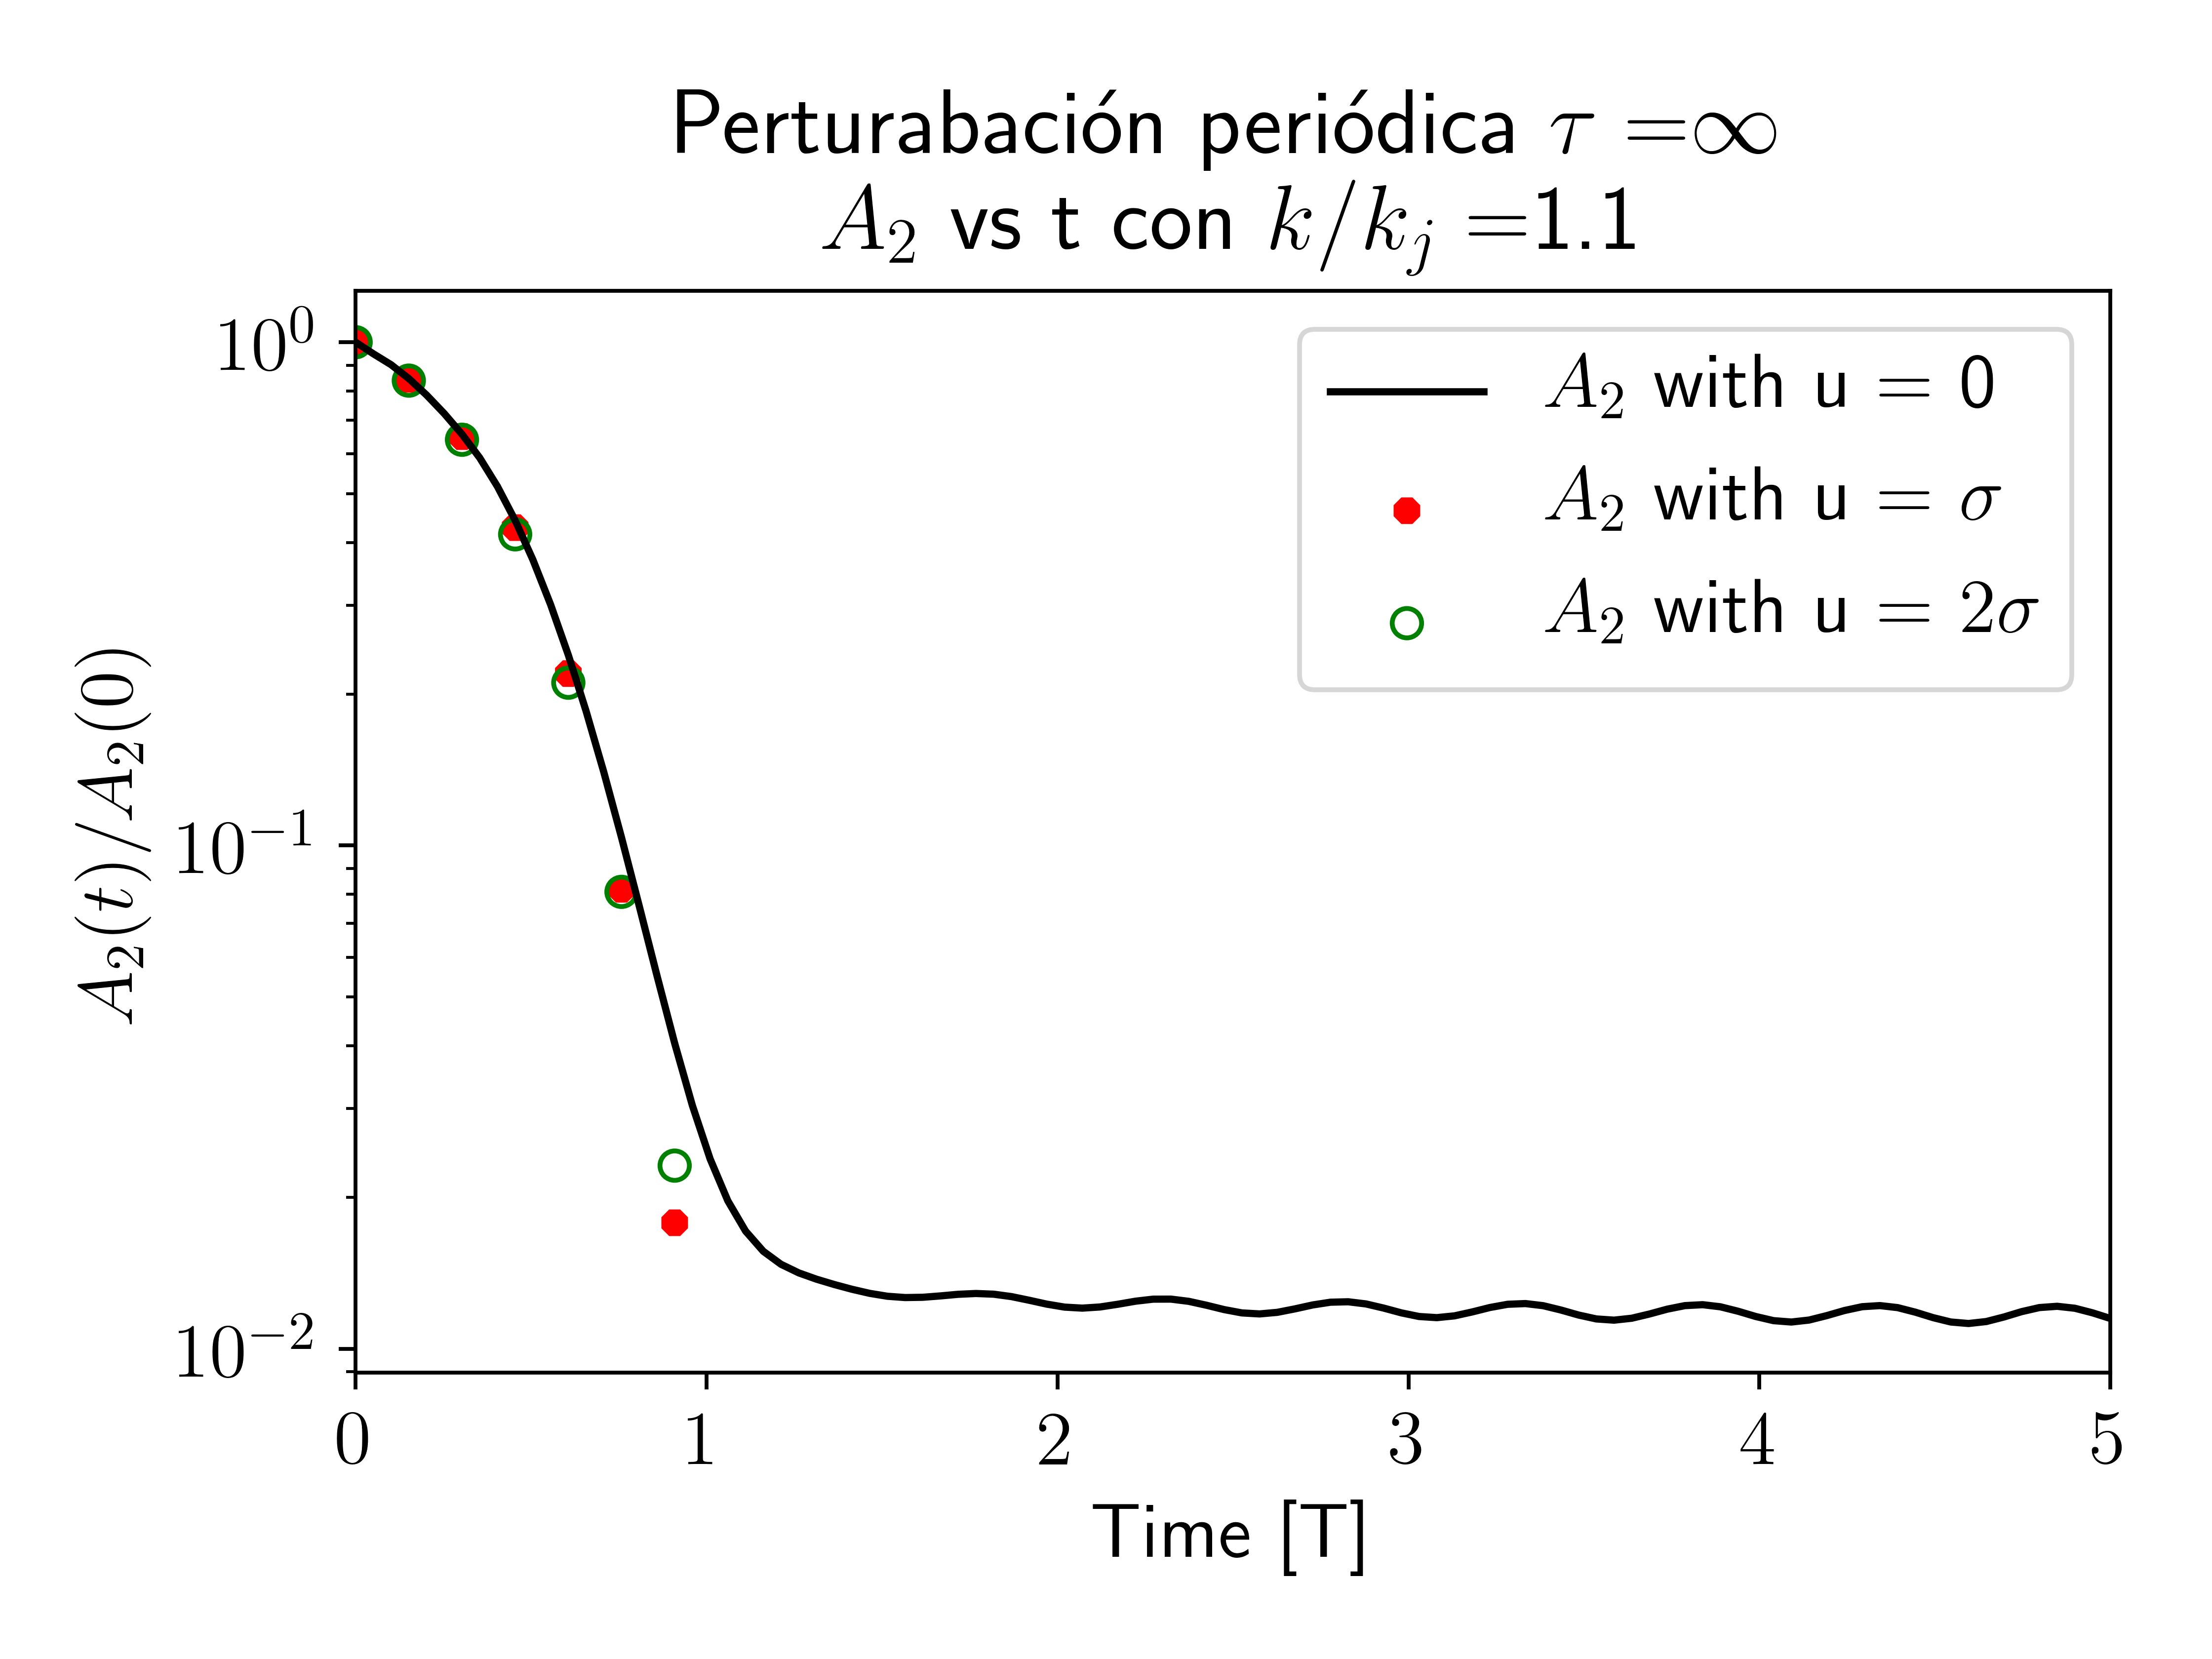
\includegraphics[scale= 0.8]{Jeans2Coef.png}

  \label{fig: cobre}
\end{figure}

\begin{figure}[h]
  \centering
   \includegraphics[scale= 0.8]{jairos.png}
  \caption{Gráfica del periodo de la pulsación para diferentes razones entre las frecuencias naturales utilizando una pesa de 200g. Es de resaltar que el pico no está centrado en 1 pero está bastante cerca. Esto probablemente se debe a errores a la hora de medir la longitud de los péndulos.}
  \label{fig: cobre}
\end{figure}
